\documentclass{article}
\usepackage[spanish]{babel}
	\deactivatetilden
\spanishdecimal{.}
\addto\captionsspanish{\def\tablename{Tabla}}
\addto\captionsspanish{\def\listtablename{\'Indice de tablas}}
\usepackage[numbers,sort&compress]{natbib}
\usepackage[T1]{fontenc}
\usepackage[utf8]{inputenc}
\usepackage{graphicx}
\usepackage{url}
\usepackage{graphicx}
\graphicspath{{Figuras/}}
\usepackage[numbers,sort&compress]{natbib}
\usepackage[clearempty,pagestyles]{titlesec}
\usepackage{anysize}
\usepackage{xcolor, colortbl}
\usepackage{array, multirow, multicol}
\usepackage{enumerate} 

\def\baselinestretch{1.5}
\papersize{27.9cm}{21.5cm} 
\marginsize{2cm}{2cm}{1cm}{1cm}

\title {Método Monte-Carlo}
\author{Julio Garc\'ia}
\pagestyle{empty}

\pagestyle{empty}

\begin{document}
	\renewcommand{\listtablename}{Índice de tablas}
	\renewcommand{\tablename}{Cuadro}
\maketitle
	
\section{Introducción}
En el presente trabajo se busca como objetivo principal el estudio el método de Monte-Carlo como método de aproximación.
En la tarea de la práctica 5 \cite{p5} se busca estudiar el efecto que tiene el aumento de cifras de precisión con respecto a un target (en este caso el estimado de la integral que arroja Wolfram Alpha) en el número de iteraciones necesarias para tener una estimación con esa precisión.

\section{Desarrollo}
En este trabajo se estudia la cantidad de iteraciones (generación de aleatorios necesarios) para estimar el valor de una integral con respecto al valor arrojado por Wolfram Alpha, que en este caso es de $0.0488341$. 
Cabe mencionar que el respetar, por ejemplo, la primer cifra significativa de decimales de este número implica que un resultado entre $0.0999999$ y $0.0$, ósea se tendría un rango hacia arriba de aproximadamente $0. 0.0511658$ y hacia debajo de aproximadamente $0.0488341$. Con el fin de evitar cálculos de cotas hacia arriba y hacia abajo al cambiar los decimales que se quieren respetar se optó por la siguiente regla: si se quiere cuidar el primer decimal se le dará un rango de diferencia de 1 décimo de unidad; si se quiere cuidar dos decimales se le dará un rango de 1 centésimo de diferencia; 3 decimales 1 milésimo y así sucesivamente hasta los 7 decimales. 

\section{Experimentación y resultados}
En esta sección se describe el ambiente computacional y los resultados obtenidos con la simulación. El código de dicha simulación fue realizado en el lenguaje computacional R por ser más simple el código y por el comentario de la Dra. Elisa de que al parecer el generador de R es un poco más refinado, en una computadora personal con procesador 1 Intel Core i7, con memoria RAM de $16$ GB y hasta 8 núcleos de procesamiento. Dicho código fue incorporado en el repositorio \cite{p_5}.
Cabe mencionar que como se busca una cota para la cantidad de números pseudoaleatorios que se deben de generar para tener una aproximación adecuada de la integral, se le quitó la parte de paralelizar ya que en cada iteración se requiere evaluar si ya se alcanzó el objetivo.
La experimentación consiste en realizar 10 veces la aproximación de la integral por cada cantidad de dígitos significativos que se desean cuidar. En total se realizaron 70 corridas quedando los resultados como se presentan a continuación:


\begin{table}[htbp]
	\centering
	\caption{Decimales significativos vs Cantidad de iteraciones}
	\begin{tabular}{|c|c|c|c|c|c|c|c|}
		\hline
		& \multicolumn{7}{c|}{Decimales Significativos} \\
		\hline
		& \multicolumn{1}{l|}{1 decimal} & \multicolumn{1}{l|}{2 decimales} & \multicolumn{1}{l|}{3 decimales} & \multicolumn{1}{l|}{4 decimales} & \multicolumn{1}{l|}{5 decimales} & \multicolumn{1}{l|}{6 decimales} & \multicolumn{1}{l|}{7 decimales} \\
		\hline
		& 1     & 1     & 2     & 21    & 21    & 260   & 37 \\
		\hline
		& 1     & 1     & 9     & 17    & 35    & 1456  & 1145 \\
		\hline
		& 1     & 1     & 4     & 16    & 63    & 139   & 700 \\
		\hline
		& 1     & 1     & 2     & 17    & 72    & 250   & 4613 \\
		\hline
		\multicolumn{1}{|l|}{Iteraciones} & 1     & 1     & 4     & 83    & 35    & 125   & 729 \\
		\hline
		& 1     & 1     & 1     & 122   & 7     & 352   & 777 \\
		\hline
		& 1     & 1     & 1     & 127   & 331   & 441   & 3744 \\
		\hline
		& 1     & 1     & 2     & 10    & 633   & 1846  & 4974 \\
		\hline
		& 1     & 1     & 9     & 28    & 56    & 581   & 3254 \\
		\hline
		& 1     & 1     & 2     & 8     & 39    & 84    & 7251 \\
		\hline
	\end{tabular}%
	\label{tab:addlabel}%
\end{table}%
\newpage
\begin{figure}[h]
	\centering
	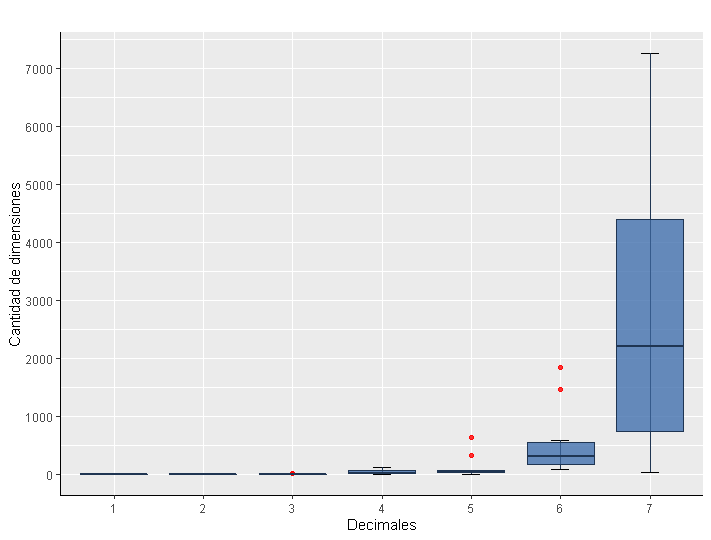
\includegraphics[width=0.6\linewidth]{Rplot03}
	\caption{Decimales significativos vs Cantidad de iteraciones}
	\label{fig:imagen2}
\end{figure}

\section{Conclusiones}
Tomando como referencia los resultados mostrados en el diagrama, con las iteraciones necesarias para estimar el valor de una integral podemos presentar las siguientes conclusiones:

\begin{enumerate}
\item Conforme se requiere mas acercamiento a un target, en este caso el resultado de Wolfram Alpha, el número de pseudoaleatorios generados por el método Monte-Carlo va a aumentando significativamente en promedio.	
\item Es importante notar que en cada ejecución hay resultados muy distinto y esto se debe a que es una muestra pseudoaleatoria, por tanto se puede alcanzar el target con el primer pseudoaleatorio generado o pueden requerirse miles de pseudoaleatorios generados. 
\end{enumerate}

\bibliography{Biblio}
\bibliographystyle{plainnat}

\end{document}

